\section{Transformation to Polygonal Dual}
\label{sect:transformation-to-dual}

In this step of the pipeline, we take a filtered cluster graph \clustergraph{} and form a polygonal dual of thereof, resulting in the map \initmap{}.
To formalize the their relationship, we need the concept of the augmented dual:

\begin{definition}
The \emph{augmented dual} $G^+$ of a plane graph $G$ is the plane multigraph obtained by first placing a new vertex $v^+$ in the outer face of $G$, connecting it to all vertices on the outer face, in order, without introducing edge crossings, and then forming its dual.
\label{def:augmented-dual}
\end{definition}

\Cref{fig:transformation-augmented-dual} illustrates how the augmented dual $G^+$ of a plane graph $G$ (\cref{subfig:transformation-augmented-dual-1}) is formed.
We add the helper vertex $v^+$ and helper edges $\{v^+,\cdot\}$ in the outer face in \cref{subfig:transformation-augmented-dual-2}.
We draw the helper edges as in \cite{wagner2016algorithmen} because it does not matter where in the plane this helper vertex lies \emdash{} all that matters is that each pair of adjacent vertices on the outer face forms a new triangular face with $v^+$.
In \cref{subfig:transformation-augmented-dual-3}, we overlay the dual vertices and edges in red.
\Cref{subfig:transformation-augmented-dual-4} shows just the augmented dual of $G$.
%
\begin{figure}[H]
	\centering
	\subfigure[]{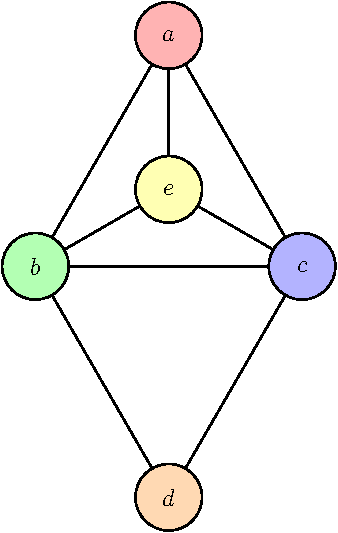
\includegraphics[height=130px]{Resources/Transformation-AugmentedDual-1.pdf}\label{subfig:transformation-augmented-dual-1}}
	\quad
	\subfigure[]{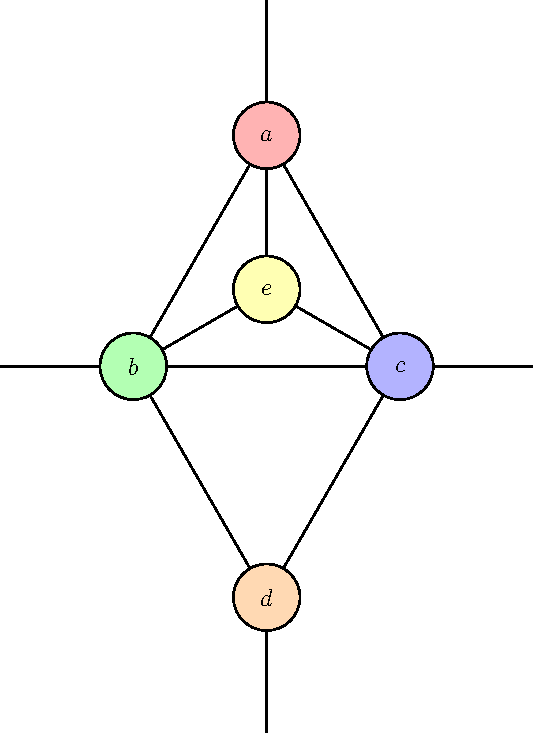
\includegraphics[height=130px]{Resources/Transformation-AugmentedDual-2.pdf}\label{subfig:transformation-augmented-dual-2}}
	\quad
	\subfigure[]{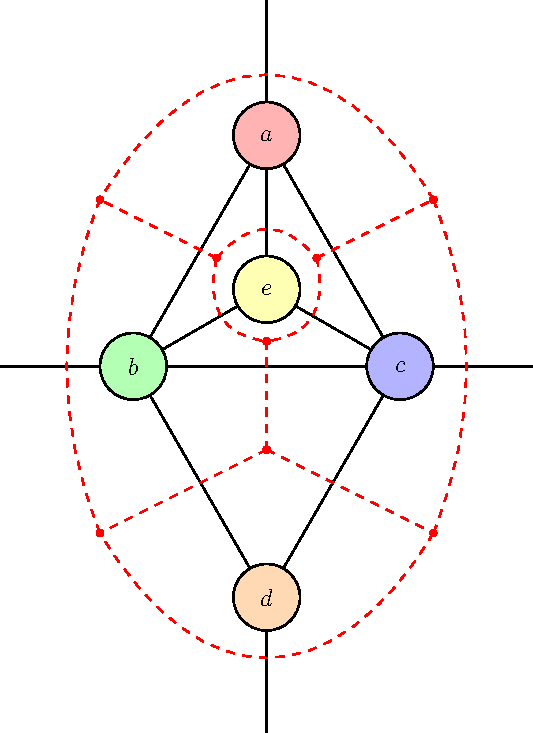
\includegraphics[height=130px]{Resources/Transformation-AugmentedDual-3.pdf}\label{subfig:transformation-augmented-dual-3}}
	\quad
	\subfigure[]{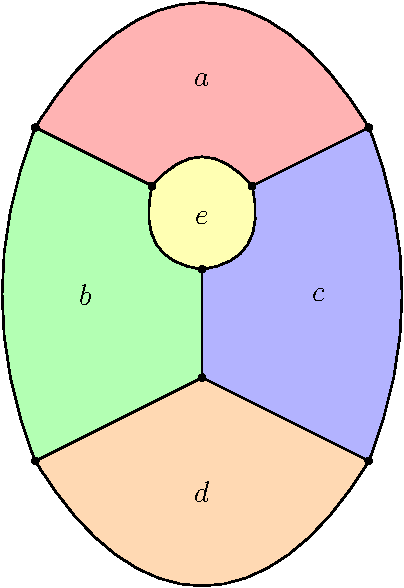
\includegraphics[height=130px]{Resources/Transformation-AugmentedDual-4.pdf}\label{subfig:transformation-augmented-dual-4}}
	\caption{Step-by-step representation of forming a plane graph's augmented dual.}
	\label{fig:transformation-augmented-dual}
\end{figure}

Note that analogous to the regular dual, the weak dual of the augmented dual of a plane graph $G$ is $G$ again, \ie{} $(G^+)^- = G$.

The augmented dual $G^+$ (\cref{subfig:transformation-augmented-dual-4}) of a biconnected and internally triangulated plane graph $G$ (\cref{subfig:transformation-augmented-dual-1}) essentially is a contact representation thereof.
In a polygonal dual, however, the edges cannot be curves and must be polylines instead.
The map \initmap{} can therefore be interpreted as a subdivision of the augmented dual $(\clustergraph{})^+$ in combination with a planar straight-line drawing thereof.



\paragraph{Algorithm Overview}

The underlying idea of creating the initial map \initmap{} is as follows:
Given a filtered cluster graph \clustergraph{}, we place vertices on edges of the outer face of \clustergraph{} (those edges bound additional triangular faces after adding the helper vertex in the process of forming the augmented dual) and inside the internal faces of \clustergraph{}.
We then connect these vertices if their corresponding faces are adjacent.
Connecting two vertices may require additional subdivision vertices or bends in order not to introduce edge crossings \emdash{} we use a single bend per edge.

The following figure illustrates an example:
%
\begin{figure}[H]
	\centering
	\subfigure[]{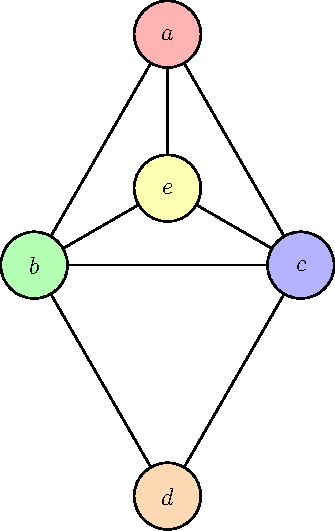
\includegraphics[height=70mm]{Resources/Transformation-Algorithm-1.pdf}\label{subfig:transformation-algorithm-1}}
	\quad
	\subfigure[]{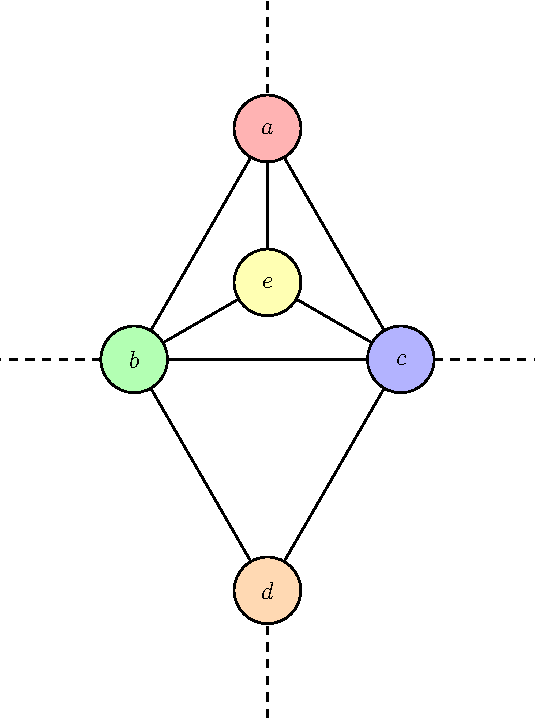
\includegraphics[height=70mm]{Resources/Transformation-Algorithm-2.pdf}\label{subfig:transformation-algorithm-2}}
	\quad
	\subfigure[]{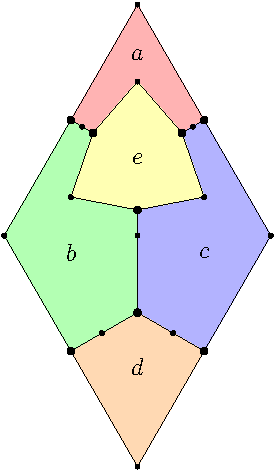
\includegraphics[height=70mm]{Resources/Transformation-Algorithm-3.pdf}\label{subfig:transformation-algorithm-3}}
	\caption{A filtered cluster graph \clustergraph{} (a), the helper graph \clustergraph{+} (b), and the polygonal dual \initmap{} of \clustergraph{} as produced by \cref{alg:transformation-to-dual} (c).}
	\label{fig:transformation-algorithm}
\end{figure}

Before feeding the filtered cluster graph \clustergraph{} into the algorithm, we construct a planar straight-line drawing \clusterdrawing{} of \clustergraph{} with the same planar embedding.
According to Fáry's theorem \cite{fary1948straight} \cite{wagner1936bemerkungen} \cite{stein1951convex}, such a drawing exists for every plane graph.
There are numerous popular algorithms to construct such a drawing, \eg{} Tutte's method \cite{tutte1963draw}, the shift method \cite{fraysseix1990draw}, or the Schnyder realizer method \cite{schnyder1990embedding}.



\clearpage
\paragraph{Algorithm Implementation}

\begin{algorithm}[H]
  \caption{Transformation to Polygonal Dual}
  \label{alg:transformation-to-dual}
  \SetKwData{Endpoints}{endpoints}
  \SetKwFunction{Appending}{appending}
  \SetArgSty{textrm}
  \vspace{5pt}
  \KwData{filtered cluster graph \clustergraph{} and a planar straight-line drawing \clusterdrawing{} thereof}
  \KwResult{polygonal dual \initmap{} of \clustergraph{}, in the form of a 1-subdivision of the augmented dual of \clustergraph{} and planar straight-line drawing thereof}
  \vspace{10pt}
  create empty contact representation \initmap{}\;
  \ForEach{internal face $f$ in \clustergraph{}}{
    \label{line:transformation-loop1-start}
    add \quoted{internal face vertex} $v_f$ to \initmap{}\; \label{line:transformation-innerfacevertex}
    position $v_f$ at barycenter of $f$ in \clustergraph{} \label{line:transformation-barycenter1}\;
    \label{line:transformation-loop1-end}
  }
  \ForEach{edge $\{u,v\}$ in \clustergraph{}}{
    \label{line:transformation-loop2-start}
  	\If{$\{u,v\}$ is incident to two different internal faces $f, g$ in \clustergraph{} \label{line:transformation-incidentfacelookup1}}{
  	  add \quoted{subdivision vertex} $v_\text{sub}$ to \initmap{}\; \label{line:transformation-subdivisionvertex1}
  	  position $v_\text{sub}$ at midpoint of ${\{u,v\}}$ in \clustergraph{}\;
  	  add edge between $v_f$ and $v_\text{sub}$ to \initmap{}\; \label{line:transformation-edgetype1-start}
  	  add edge between $v_\text{sub}$ and $v_g$ to \initmap{}\; \label{line:transformation-edgetype1-end}
  	}
  	\ElseIf{$\{u,v\}$ is incident to a single internal face $f$ in \clustergraph{} \label{line:transformation-incidentfacelookup2}}{
  	  add \quoted{outer edge vertex} $v_{\{u,v\}}$ to $G_\text{init}$\; \label{line:transformation-outeredgevertex}
  	  position $v_{\{u,v\}}$ at midpoint of ${\{u,v\}}$ in \clustergraph{}\;
  	  add \quoted{subdivision vertex} $v_\text{sub}$ to \initmap{}\; \label{line:transformation-subdivisionvertex2}
  	  position $v_\text{sub}$ at midpoint of segment between barycenter of $f$ and midpoint of ${\{u,v\}}$ in \clustergraph{} \label{line:transformation-barycenter2}\;
  	  add edge between $v_{\{u,v\}}$ and $v_\text{sub}$ to \initmap{}\; \label{line:transformation-edgetype2-start}
  	  add edge between $v_\text{sub}$ and $v_f$ to \initmap{}\; \label{line:transformation-edgetype2-end}
  	}
  	\label{line:transformation-loop2-end}
  }
  \ForEach{incident edges $\{\{u,v\},\{v,w\}\}$ on outer face of \clustergraph{}}{
    \label{line:transformation-loop3-start}
    add \quoted{subdivision vertex} $v_\text{sub}$ to \initmap{}\; \label{line:transformation-subdivisionvertex3}
    position $v_\text{sub}$ at position of $v$ in \clustergraph{}\;
    add edge between $v_{\{u,v\}}$ and $v_\text{sub}$ to \initmap{}\; \label{line:transformation-edgetype3-start}
    add edge between $v_\text{sub}$ and $v_{\{v,w\}}$ to \initmap{}\; \label{line:transformation-edgetype3-end}
    \label{line:transformation-loop3-end}
  }
  \ForEach{vertex $u$ in \clustergraph{} \label{line:transformation-enumeratevertices}}{
    \label{line:transformation-loop4-start}
    $\Endpoints \gets ()$\;
    \ForEach{adjacent pair $(v,w)$ of neighbors of $u$ in counterclockwise order \label{line:transformation-enumerateedges}}{
      \If{$(u,v,w)$ bound a triangular face $f$ in counterclockwise order in \clustergraph{} \label{line:transformation-checktriangle}}{
        append $v_f$ to \Endpoints\;
      }
      \Else{
        append $v_{\{u,v\}}$ to \Endpoints\;
        append $v_{\{u,w\}}$ to \Endpoints\;
      }
    }
    \ForEach{adjacent pair $(v,w)$ in \Endpoints \label{line:transformation-insertsubdivisions}}{
      insert subdivision vertex connecting $v$ to $w$ between $v$ and $w$ in \Endpoints\;
    }
    define $f_u$ as internal face on \Endpoints in \initmap{}\;
    set weight of $f_u$ in \initmap{} to weight of $u$ in \clustergraph{}\;
    \label{line:transformation-loop4-end}
  }
  \Return \initmap{}
\end{algorithm}
\vfill



\paragraph{Algorithm Correctness}

We show the algorithm's correctness in two steps.
First, we show that the algorithm does indeed construct a 1-subdivision of the augmented dual of \clustergraph{}.
Second, we show that the constructed drawing thereof is planar, making it a contact representation of \clustergraph{} as previously explained and illustrated in \cref{fig:transformation-augmented-dual}.

Recall that $(\clustergraph{})^+$ is a contact representation of \clustergraph{}.
We can construct $(\clustergraph{})^+$ via a helper graph \clustergraph{+} that we obtain by inserting a helper vertex $v_+$ in the outer face of \clustergraph{} and connecting it to all vertices on the outer face of \clustergraph{}, in order, without introducing edge crossings.
The contact representation $(\clustergraph{})^+$ then is the regular dual of \clustergraph{+}, \ie{} $(\clustergraph{})^+ = (\clustergraph{+})^*$.
By adding the helper vertex $V_+$ and helper edges $\{v,\cdot\}$, the edges on the outer face of \clustergraph{} bound new triangular faces of \clustergraph{+}.

The dual of a plane graph has vertices in each of the primal graph's faces.
We place these vertices in the original internal faces in \cref{line:transformation-innerfacevertex} and in \emdash{} or rather on \emdash{} the new triangular faces in \clustergraph{+} in \cref{line:transformation-outeredgevertex}.
Vertices in the dual are adjacent if their respective faces are adjacent in the primal.
Thus for every edge separating two faces in the primal \clustergraph{+}, we require a dual edge in $(\clustergraph{+})^*$.
We add these edges in \crefrange{line:transformation-edgetype1-start}{line:transformation-edgetype1-end} (for adjacent internal faces in \clustergraph{}), in \crefrange{line:transformation-edgetype2-start}{line:transformation-edgetype2-end} (for edges separating an internal face in \clustergraph{} from a new face in \clustergraph{+}), and in \crefrange{line:transformation-edgetype3-start}{line:transformation-edgetype3-end} (for helper edges $\{v_+,\cdot\}$ separating two new faces in \clustergraph{+}).
Because we place all bends of the dual edges on the respective primal edge, the cyclic order of the edges incident to each vertex is equivalent to the cyclic order of the edges bounding the respective faces in the primal.

\begin{figure}[H]
	\centering
	\subfigure[]{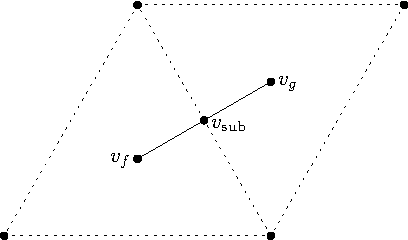
\includegraphics[height=32mm]{Resources/Transformation-DualEdgeConstruction-1.pdf}\label{subfig:transformation-dual-edge-construction-1}}
	\subfigure[]{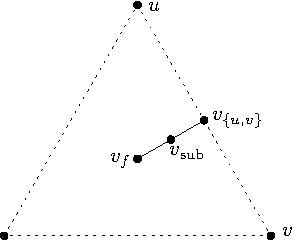
\includegraphics[height=32mm]{Resources/Transformation-DualEdgeConstruction-2.pdf}\label{subfig:transformation-dual-edge-construction-2}}
	\quad
	\subfigure[]{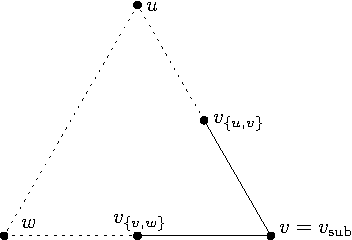
\includegraphics[height=32mm]{Resources/Transformation-DualEdgeConstruction-3.pdf}\label{subfig:transformation-dual-edge-construction-3}}
	\caption{Construction of the dual edges as per \cref{alg:transformation-to-dual} between two internal faces in \clustergraph{} (a), between an internal face of \clustergraph{} and a new face in \clustergraph{+} (b), and between two new faces in \clustergraph{+} (c). The dotted lines are edges in \clustergraph{}.}
	\label{fig:transformation-dual-edge-construction}
\end{figure}

It is left to show that the placement of vertices and edges produces a crossing-free drawing.
To do so, we consider the edges from non-subdivision vertices in $(\clustergraph{+})^*$ to their neighbors.
Recall that those vertices correspond to faces in \clustergraph{+}.
Following the construction illustrated in \crefrange{subfig:transformation-dual-edge-construction-1}{subfig:transformation-dual-edge-construction-2}, the three incident edges to a vertex corresponding to an internal face of \clustergraph{} lie completely inside said face.
Because these edges go straight towards the midpoint of the incident edges, they don't self-intersect.

The vertices corresponding to new faces in \clustergraph{+} lie on the midpoint of the bounding edge that already exists in \clustergraph{}.
The dual edges connecting two of those vertices are constructed such that they partition the boundary of the outer face of \clustergraph{} (see \cref{subfig:transformation-dual-edge-construction-3}) and therefore don't intersect any of the edges discussed so far.
Their edge to the vertex corresponding to the adjacent internal face goes straight towards said vertex, meeting it halfway, as illustrated in \cref{subfig:transformation-dual-edge-construction-2}.
Because some $v_f$'s incident edges all go straight towards its bounding edges as outlined above, this kind of edge does not introduce any edge crossings either.
The constructed graph and drawing is therefore a 1-subdivision of the augmented dual of \clustergraph{} and the drawing is planar.

Once the algorithm has constructed \initmap{}, we compute an explicit representation of its internal faces and the corresponding vertices in the primal.
We do so for the augmented dual $(\clustergraph{})^+$ first (loop in \cref{line:transformation-enumerateedges}) and then insert the subdivision vertices (loop in \cref{line:transformation-insertsubdivisions}).
The face in $(\clustergraph{})^+$ that corresponds to a vertex $v$ of \clustergraph{} is bounded by vertices corresponding to internal faces of \clustergraph{} that contain $v$, plus the vertices corresponding to the additional triangular faces in \clustergraph{+} in case $v$ lies on outer face of \clustergraph{}.
Iterating over adjacent pairs $(e_1, e_2)$ of incident edges in counterclockwise order correctly detects the internal faces between $e_1$ and $e_2$ and the case where $e_1$ and $e_2$ wrap around on the outside, in order.
The orientation check in \cref{line:transformation-checktriangle} is required such that the wraparound case isn't misclassified as an internal face.
This would be the case for internal faces of \clustergraph{} with two edges on the outer face, as is the case for vertex $v \coloneqq d$ and edges $e_1 \coloneqq \{d,b\}, e_2 \coloneqq \{d,c\}$ in \cref{fig:transformation-algorithm}.



\paragraph{Algorithm Runtime}

To compute the input graph's faces, we replace every edge with two inversely oriented, directed edges.
We then repeatedly pick any unmarked edge and form a directed cycle by following the next outgoing edge according to the embedding, marking the edges as we go.
Once all edges have been marked, we have found all faces.
The outer face is the one face whose interior is on the left when traveling along its bounding edges.
This can be implemented in $\bigTheta{n+m}$, where $n = \lvert V(\clustergraph{}) \rvert$ and $m = \lvert E(\clustergraph{}) \rvert$.

The input graph has $\bigTheta{n}$ internal faces and they are all triangles, therefore we can compute their barycenter in $\bigTheta{1}$ each (\cref{line:transformation-barycenter1}, \cref{line:transformation-barycenter2}).
By keeping track of of which faces an edge of the input graph is incident to while computing the faces as outlined above, we allow for $\bigTheta{1}$ lookups in \cref{line:transformation-incidentfacelookup1} and \cref{line:transformation-incidentfacelookup2}.
The loop in \crefrange{line:transformation-loop1-start}{line:transformation-loop1-end} therefore runs in $\bigTheta{n}$, the loop in \crefrange{line:transformation-loop2-start}{line:transformation-loop2-end} in $\bigTheta{m}$, and the loop in \crefrange{line:transformation-loop3-start}{line:transformation-loop3-end} in $\bigTheta{m}$.

The loop in \crefrange{line:transformation-loop4-start}{line:transformation-loop4-end} processes every vertex once in \cref{line:transformation-enumeratevertices} and and every edge twice \cref{line:transformation-enumerateedges}.
We can check if the vertices $u,v,w$ form a triangle in constant time (\cref{line:transformation-checktriangle}) by checking if there's an edge between $v$ and $w$.
Considering each of the $\bigTheta{n+m}$ vertices of the generated graph appears in \code{endpoints} in no more than two iterations of the loop in \crefrange{line:transformation-loop4-start}{line:transformation-loop4-end} and all those vertices have degree 3, we can find their shared neighbor in constant time and implement the entire loop to run in $\bigTheta{n+m}$.

The entire algorithm can therefore be implemented to run in $\bigTheta{n+m}$.



\paragraph{Theoretical Bounds}

But do we have to subdivide edges of the augmented dual of our filtered cluster graph \clustergraph{} in order to get a valid polygonal dual of \clustergraph{}?
Although the augmented dual $(\clustergraph{})^+$ is plane by definition, it is not immediately obvious that there exists a planar straight-line drawing of $(\clustergraph{})^+$ \emdash{} and that's what we need for it to be a polygonal contact representation.

In our case, however, $(\clustergraph{})^+$ is simple, \ie{} there are no loops or multiple adjacencies.
Recall that \clustergraph{} is biconnected and internally triangulated.
Adding the helper vertex in the outer face of \clustergraph{} and connecting it to all vertices on the outer face therefore creates a fully triangulated, simple graph.
In a simple triangulated graph, there are no two edges that are incident to the same faces (only those would create multiple adjacencies when forming the dual) and no edges that have the same face on both sides (only those would create loops when forming the dual) either.
The augmented dual $(\clustergraph{})^+$ is therefore simple and, according to Fáry's theorem \cite{fary1948straight}, there exists a planar straight-line drawing of $(\clustergraph{})^+$ respecting its original planar embedding.

In addition to having a planar straight-line drawing, $(\clustergraph{})^+$ is also a cubic graph, \ie{} one in which all vertices have degree 3.
This is because \clustergraph{} with the helper vertex is a triangulated graph, meaning every face is incident to exactly three edges, which turns into every vertex being incident to exactly three edges when forming the dual.
According to the results of Thomassen \cite{thomassen1992plane}, $(\clustergraph{})^+$ is therefore area-universal.
This means that regardless of the concrete face weights that \clustergraph{} prescribes, there exists a planar straight-line drawing of $(\clustergraph{})^+$ realizing those weights/areas.

Even without subdividing edges in $(\clustergraph{})^+$, we could therefore choose the map \initmap{} in such a way that it has perfect statistical accuracy already.
Such a drawing of $(\clustergraph{})^+$ is non-trivial to compute though and creates undesired region shapes according to our other quality metrics.
Instead, the algorithm we proposed here subdivides all edges of the augmented dual $(\clustergraph{})^+$ once and leaves us with a decent initial drawing and enough degrees of freedom to optimize for other quality metrics in \cref{sect:drawing-the-dual}.
